%&latex
%
\documentclass[../template.tex]{subfiles}
\usepackage{graphicx}

\begin{document}

\section{Review of Mathematical Methods}
\subsection{Continuous Random Variables}
Let $X$ be a \textit{continuous} random variable with probability distribution $p(x)$. Then:
\begin{itemize}
    \item The probability of $X$ assuming values in the interval $[a,b)$ is given by:
    \begin{align*}
        \mathbb{P}[a \leq X < b] = \int_a^b p(x) \dd{x}
    \end{align*}
    \item The probability distribution $p(x)$ represents the \textit{infinitesimal} probability of $X$ assuming a value \textit{very close to} $x$:
    \begin{align*}
        \mathbb{P}(x \leq X < x+ \dd{x}) = p(x) \dd{x}
    \end{align*} 
    \item The expected value of a function of $X$ (also called an \textbf{observable}) $O(X)$ is given by sampling many $X_i \sim p$ all \textbf{independently} and \textbf{identically}, and then computing the limit:
    \begin{align*}
        \langle O \rangle &= \lim_{n \to \infty} \frac{1}{n} \sum_{i=1}^n O(X_i) =\\
        &= \int_{\mathbb{R}} p(x) O(x) \dd{x} \equiv \mathbb{E}[O(X)]
    \end{align*}  
    Physically, this corresponds to \textit{repeating many time the same measurement of $O$}, and averaging the results.
\end{itemize}

\begin{exo}[Some example distributions]\label{ex:dist-moments}
    Consider the following distributions:
    \begin{subequations}\label{eqn:example-dist}
        \begin{alignat}{2} \label{eqn:uniform-dist}
            &\text{\textbf{Uniform}} &\quad p_1(x) &= \begin{cases}
                1 & 0 \leq x \leq 1\\
                0 & \text{otherwise}
            \end{cases} \\ \label{eqn:exponential-dist}
            &\textbf{Exponential} &\quad p_2(x) &= \frac{1}{m} \exp\left(-\frac{x}{m} \right) \theta(x); \qquad \theta(x) = \begin{cases}
                1 & x > 0\\
                0 & x < 0
            \end{cases}\\ \label{eqn:gaussian-dist}
            &\textbf{Gaussian}  &\quad p_3(x) &=\frac{1}{\sigma \sqrt{2 \pi}} \exp\left(-\frac{(x-m)^2}{2 \sigma^2} \right) 
        \end{alignat}
    \end{subequations}

    Evaluate $\langle X \rangle$, $\langle X^2 \rangle$ and $\operatorname{Var}(X) = \langle X^2 \rangle - \langle X \rangle^2$ with the above three distributions (\ref{eqn:uniform-dist}-\ref{eqn:gaussian-dist}). Are the three distributions correctly normalized, that is:
    \begin{align*}
        \int_{\mathbb{R}} p_i(x) \dd{x} \overset{?}{=}  1 \qquad \forall i=1,2,3
    \end{align*}

    \medskip

    \textbf{Solution}. 
    \begin{enumerate}
        \item The distribution is already normalized:
        \begin{align*}
            \int_\mathbb{R} p_1(x) \dd{x} = \int_0^1 1 \dd{x} = 1
        \end{align*}
        The first two moments are:
        \begin{align*}
            \langle X \rangle &= \int_{\mathbb{R}} x\, p_1(x) = \int_0^1 x \dd{x} = \frac{x^2}{2} \Big|_0^1 = \frac{1}{2}  \\
            \langle X^2 \rangle &= \int_{\mathbb{R}} x^2 p_1(x) = \int_0^1 x^2 \dd{x} = \frac{x^3}{3} \Big|_0^1 = \frac{1}{3} 
        \end{align*}
        And so the variance can be computed as:
        \begin{align*}
            \operatorname{Var}(X) = \langle X^2 \rangle - \langle X \rangle^2 = \frac{1}{3} - \frac{1}{4} = \frac{1}{12}   
        \end{align*}
        \item We proceed exactly in the same way:
        \begin{align*}
            \int_{\mathbb{R}} p_2(x) \dd{x} = \int_0^{+\infty} \frac{1}{m}\exp\left(-\frac{x}{m} \right) \dd{x}= - \exp\left(-\frac{x}{m} \right) \Big|_0^{+\infty} = 1 \span\\
            \langle X \rangle &= \int_\mathbb{R} x\,p_2(x) \dd{x}= \int_0^{+\infty} \frac{x}{m} \exp\left(-\frac{x}{m} \right) \underset{(a)}{\dd{x}=} \\
            &=\cancel{ -x \exp\left(-\frac{x}{m} \right) \Big|_0^{+\infty} }+ \int_0^{+\infty} \exp\left(-\frac{x}{m} \right) \dd{x}= -m \exp\left(-\frac{x}{m} \right)\Big|_0^{+\infty} = m\\
            \langle X^2 \rangle &= \int_{\mathbb{R}} x^2\,p_2(x) = \int_0^{+\infty} \frac{x^2}{m} \exp\left(-\frac{x}{m} \right)  \dd{x} \underset{(b)}{=} \\
            &= \cancel{-x^2 \exp\left(-\frac{x}{m} \right) \Big|_0^{+\infty}} -\cancel{2m x \exp\left(-\frac{x}{m} \right)\Big|_0^{+\infty} }+2m \int_0^{+\infty} \exp\left(-\frac{x}{m} \right)\dd{x} =\\
            &=-2m^2 \exp\left(-\frac{x}{m} \right)\Big|_0^{+\infty} = 2m^2\\
            \operatorname{Var}(X) &= \langle X^2 \rangle - \langle X \rangle^2 = 2m^2 - m^2 = m^2
        \end{align*}
        where in (a) and (b) we performed (multiple) integrations by parts.
        \item As before:
        \begin{align*}
            \int_\mathbb{R} \frac{1}{\sigma \sqrt{2 \pi}} \exp\left(-\frac{(x-m)^2}{2 \sigma^2} \right)\dd{x}\> \underset{\mathclap{y=\frac{x-m}{\sqrt{2}\sigma}}}{=} \quad \int_{\mathbb{R}} \frac{\dd{y}}{\sqrt{ \pi}} e^{-y^2} = \frac{\sqrt{\pi}}{\sqrt{\pi}} = 1 \span \\
            \langle X \rangle &= \int_{\mathbb{R}} \frac{x}{\sigma \sqrt{2 \pi}} \exp\left(-\frac{(x-m)^2}{2 \sigma^2} \right) \dd{x} = \int_{\mathbb{R}} \frac{\sqrt{2} \sigma y + m}{\sqrt{\cancel{2} \pi} \cancel{\sigma}} e^{-y^2} \cancel{\sqrt{2} \sigma }\dd{y} =\\
            &\underset{(a)}{=}  \frac{m}{\sqrt{\pi}}  \int_{\mathbb{R}} e^{-y^2} = m
            \shortintertext{In (a) we noted that the $y e^{-y^2}$ term is an \textit{odd} function integrated over a symmetric domain, and so it vanishes.}\\
            \langle X^2 \rangle &= \int_{\mathbb{R}} \frac{x^2}{\sqrt{2\pi} \sigma} \exp\left(-\frac{(x-m)^2}{2 \sigma^2} \right) \dd{x} =  \int_{\mathbb{R}} \frac{(\sqrt{2} \sigma y + m)^2}{\sqrt{\cancel{2} \pi} \cancel{\sigma}} e^{-y^2} \cancel{\sqrt{2} \sigma }\dd{y} =\\
            &= \int_{\mathbb{R}} \frac{2 \sigma^2}{\sqrt{\pi}} y^2 e^{-y^2} \dd{y} +\cancel{ \int_{\mathbb{R}} \frac{2 \sqrt{2} \sigma m}{\sqrt{\pi}} y e^{-y^2} \dd{y}} + m^2 \int_{\mathbb{R}} \frac{1}{\sqrt{\pi}} e^{-y^2} \dd{y} =\\
            &= \frac{2 \sigma^2}{\sqrt{\pi}} \int_{\mathbb{R}} y^2 e^{-y^2} \dd{y} + m^2
        \end{align*}
        For the last integral, we note that:
        \begin{align*}
            \int_{\mathbb{R}} y^2 e^{-y^2}\dd{y} = - \dv{s} \int_{\mathbb{R}} e^{-sy^2} \dd{y} \Big|_{s=1}
        \end{align*}
        and:
        \begin{align*}
            \int_{\mathbb{R}} e^{-sy^2}\dd{y} \underset{t = \sqrt{s}y}{=}  \int_{\mathbb{R}} \frac{\dd{t}}{\sqrt{s}} e^{-t^2} = \sqrt{\frac{\pi}{s}} 
        \end{align*}
        meaning that:
        \begin{align*}
            \int_{\mathbb{R}} e^{-y^2} e^{-y^2} = -\dv{s} \sqrt{\frac{\pi}{s} } \Big|_{s=1} = \frac{\sqrt{\pi}}{2} s^{-3/2} \Big|_{s=1} = \frac{\sqrt{\pi}}{2} 
        \end{align*}
        Substituting in the previous expression we finally get:
        \begin{align*}
            \langle X^2 \rangle &= \frac{\bcancel{2} \sigma^2}{\sqrt{\cancel{\pi}}} \frac{\sqrt{\cancel{\pi}}}{\bcancel{2}} + m^2 = \sigma^2 + m^2 \\
            \operatorname{Var}(X) &= \langle X^2 \rangle - \langle X \rangle^2 = \sigma^2
        \end{align*}
    \end{enumerate}
     
\end{exo}

\begin{exo}[Variance properties]
    Show that:
    \begin{enumerate}
        \item $\operatorname{Var}(X) \equiv \langle (X-\langle X \rangle)^2 \rangle = \langle X^2 \rangle - \langle X^2 \rangle$
        \item $\displaystyle \min_a \langle (X-a)^2 \rangle = \operatorname{Var}(X)$ with $a \in \mathbb{R}$ 
    \end{enumerate}
    
    \medskip

    \textbf{Solution}.
    \begin{enumerate}
        \item By using the linearity of the average:
        \begin{align*}
            \operatorname{Var}(X) &= \langle (X - \langle X \rangle)^2 \rangle = \langle X^2 -  2 X \langle X \rangle + \langle X \rangle^2\rangle = \\
            &=\langle X^2 \rangle - 2 \langle X \rangle \langle X \rangle + \langle X \rangle^2 = \langle X^2 \rangle - \langle X \rangle^2
        \end{align*}
        \item First we expand the square, and use again the linearity of the average:
        \begin{align*}
            \langle (X-a)^2 \rangle = \langle X^2 \rangle - 2a \langle X \rangle + a^2
        \end{align*}
        To \textit{minimize} this expression, we differentiate wrt $a$ and set the derivative to $0$:
        \begin{align*}
            \dv{a} [\langle X^2 \rangle -2a \langle X \rangle + a^2] = -2 \langle X \rangle + 2a \overset{!}{=} 0 \Rightarrow a = \langle X \rangle
        \end{align*} 
        And substituting in the expression above we have:
        \begin{align*}
            \min_a \langle (X-a)^2 \rangle = \langle X^2 \rangle - 2 \langle X \rangle \langle X \rangle + \langle X \rangle^2 = \langle X^2 \rangle-\langle X \rangle^2 = \operatorname{Var}(X) 
        \end{align*}
    \end{enumerate}
     
\end{exo}

\begin{exo}
    Consider the following pdf:
    \begin{align*}
        p(x) = (\alpha + 1) x^{-\alpha} \theta(x-1)
    \end{align*}
    For what values of $\alpha \in \mathbb{R}$ is it normalizable? Which moments $\langle x^k \rangle$, with $k \in \mathbb{R}$, are well defined?

    \medskip

    \textbf{Solution}. We start by checking the normalization:
    \begin{align*}
        \int_{\mathbb{R}} p(x) \dd{x} = \int_1^{+\infty} (\alpha + 1) x^{-\alpha} \dd{x}
    \end{align*} 
    If $\alpha =1$:
    \begin{align*}
        \int_{1}^{+\infty} \frac{1}{x} \dd{x} = \ln x \Big|_1^{+\infty} = +\infty 
    \end{align*}
    If $\alpha \neq 1$:
    \begin{align*}
        \int_1^{+\infty} \frac{1}{x^\alpha} \dd{x} = \frac{1}{1 - \alpha} x^{1 - \alpha} \Big|_{1}^{+\infty} = \begin{cases}
            +\infty & \alpha < 1\\
            -\frac{1}{1-\alpha} & \alpha > 1
        \end{cases}
    \end{align*}
    And so the integral certainly converges to a non-zero value for $\alpha > 1$:
    \begin{align*}
        \int_{\mathbb{R}} p(x) \dd{x} = \frac{\alpha+1}{\alpha-1} = A  \qquad \alpha > 1
    \end{align*}
    meaning that $p(x)/A$ is normalized.

    \medskip

    Note that the integral converges also for $\alpha = -1$, where the prefactor $(\alpha + 1)$ vanishes. However, in this case the integral is $0$, and so it cannot be normalized to $1$.

    \medskip

    The $k$-th moment, with $k \in \mathbb{R}$ is given by:
    \begin{align*}
        \langle X^k \rangle = \int_1^{+\infty} (\alpha-1) x^{k - \alpha} \dd{x} \qquad \alpha > 1
    \end{align*}
    This converges if $-(k-\alpha) = -k + \alpha > 1$, i.e. if $k < \alpha-1$, to:
    \begin{align*}
        \langle X^k \rangle = -\frac{\alpha -1}{1-\alpha +k} 
    \end{align*}
\end{exo}

\subsection{Discrete Random Variables}
A discrete random variable $X$ can only assume values inside a \textit{discrete}, \textbf{countable} (or \textit{denumerable}) set $E$. The probability of $X$ assuming a value $\omega \in E$ is denoted by:
\begin{align*}
    \mathbb{P}(X=\omega) \equiv \mathbb{P}_\omega
\end{align*}
Given an observable $O(X)$, its possible outcomes are $O(X=\omega) \equiv O_\omega\quad \forall \omega \in E$, and its expected value is given by their average:
\begin{align*}
    \langle O(X) \rangle = \sum_{\omega \in E} \mathbb{P}_\omega O_\omega
\end{align*}

\begin{exo}[Examples of discrete random variables]\label{ex:moments-discrete}
    \begin{enumerate}[label=\alph*.]
        \item Let $X_i$ be a discrete random variable with only two possible values $E_i=\{0,1\}$, with probabilities:
        \begin{align*}
            \mathbb{P}(X_i=0) \equiv p; \qquad \mathbb{P}(X_i=1) = 1-p    
        \end{align*}
        Consider $n$ random variables $\{X_i\}_{i=1,\dots,n}$ that are \textbf{independently} and \textbf{identically} \textbf{distributed} like $X$ (i.i.d.). Their sum is a new discrete random variable $X$ that assumes values between $0$ and $n$ (included):
        \begin{align*}
            X = X_1 + \dots + X_n; \qquad E_n = \{0,1,\dots, n\}
        \end{align*}
        Show that:
        \begin{enumerate}[label=\roman*.]
            \item The distribution of $X$ is the \textbf{binomial distribution}:
            \begin{align} \label{eqn:binomial-dist}
                p(k) = \mathbb{P}(X=k) = {n\choose k} p^k (1-p)^{n-k}; \qquad {n\choose k} = \frac{n!}{k! (n-k)!} 
            \end{align}
            \item $p(k)$ so defined is properly normalized:
            \begin{align*}
                \sum_{k=0}^n \mathbb{P}(X=k) = 1
            \end{align*}
            \item Evaluate $\langle X \rangle$, $\langle X^2 \rangle$, $\operatorname{Var}(X)$. 
        \end{enumerate}
        \item As before, consider a set of $n$ i.i.d. discrete random variables $\{X_i\}_{i=1,\dots,n}$, each following the same \textbf{Poisson distribution}:
        \begin{align} \label{eqn:poisson-dist}
            \mathbb{P}(X_i = k) = \frac{\lambda^k}{k!} e^{-\lambda} \quad k \in \mathbb{N}; \qquad E_i = \mathbb{N} 
        \end{align}  
        Consider their sum:
        \begin{align*}
            X=X_1 + \dots + X_n
        \end{align*}
        Show that:
        \begin{enumerate}[label=\roman*.]
            \item The distribution of the sum $X$ is:
            \begin{align*}
                \mathbb{P}(X=k) = \frac{(n \lambda)^k}{k!} e^{-n \lambda} 
            \end{align*}
            \item It is properly normalized:
            \begin{align*}
                \sum_{k=0}^{+\infty} \mathbb{P}(X=k) = 1
            \end{align*}
            \item Evaluate $\langle X \rangle$, $\langle X^2 \rangle$, $\operatorname{Var}(X)$. 
        \end{enumerate}
    \end{enumerate}

    Notice that the binomial distribution (\ref{eqn:binomial-dist}) in the case of \textit{rare events} $p=\lambda/n$ with $k \ll n$ becomes:
    \begin{align*}
        {n\choose k} p^k(1-p)^{n-k} &= \frac{n(n-1)\cdots (n-k+1)}{k!} \left(\frac{\lambda}{n} \right)^k \left(1-\frac{\lambda}{n} \right)^{n-k} \approx\\
        &\approx \frac{n^k}{k!} \left(\frac{\lambda/n}{1 - \lambda/n} \right)^k \left(1-\frac{\lambda}{n} \right)^n =\\
        &= \frac{\lambda^k}{k!}\left(1-\frac{\lambda}{n} \right)^{-k} \left(1-\frac{\lambda}{n} \right)^k =\\
        &=\frac{\lambda^k}{k!}\left[\exp\left(k \frac{\lambda}{n}+k \frac{\lambda^2}{n^2} + \dots \right) \right] \left[\exp\left(-\lambda -\frac{\lambda}{n} + \dots \right)\right] \approx\\
        &\approx \frac{\lambda^k}{k!} e^{-\lambda} 
    \end{align*} 
    which is a Poisson distribution (\ref{eqn:poisson-dist}). This argument can be made more precise using more sophisticated methods, by introducing a scalar product in the space of distributions and prove \textit{convergence in total variation}.
    
    \medskip

    \textbf{Solution}. 
    
    \begin{enumerate}
        \item $X=k$ if and only if there are exactly $k$ variables $X_i = 1$, and the others are $0$. This can happen in ${n \choose k}$ distinct ways. As the $X_i$ are independent, the probability of any configuration is just the product of the probabilities of each state. In the case we are interested on, we have always exactly $k$ states $X_i = 1$, and $n-k$ with $X_i=0$, and so the total probability of each configuration will be $p^k (1-p)^{n-k}$. Putting it all together we arrive to the binomial distribution:
        \begin{align*}
            p(k) = \mathbb{P}(X=k) = {n\choose k} p^k (1-p)^{n-k}    
        \end{align*}
        \item Applying the binomial theorem we have:
        \begin{align*}
            \sum_{k=0}^{n} \mathbb{P}(X=k) = \sum_{k=0}^{n} {n\choose k} p^k (1-p)^{n-k} = (p + [1-p])^n = 1^n = 1
        \end{align*}
        \item By direct computation:
        \begin{align*}
            \langle X \rangle &= \sum_{k=0}^{n} k\,  \mathbb{P}(X=k) = \sum_{k=0}^{n} \hlc{Yellow}{k} \frac{n!}{(n-k)!\hlc{Yellow}{ k !}} p^k(1-p)^{n-k} =\\
            &= \sum_{k=\textcolor{Red}{1}}^{n} \frac{n(n-1)!}{(n-k)!\hlc{Yellow}{(k-1)!}} p^k(1-p)^{n-k} = \\
            &= n\sum_{k=1}^{n} {n-1\choose k-1} p^k(1-p)^{n-k} =\\
            \shortintertext{Now we factor out a $p$ and sum and subtract a $1$ so that everywhere we have $k-1$:}
            &= n \textcolor{Red}{p}\sum_{k=1}^{n} {n-1\choose k-1} \textcolor{Red}{p^{k-1}} (1-p)^{(n\textcolor{Red}{-1}) - (k\textcolor{Red}{-1})}
            \shortintertext{And finally we shift the index of summation:}
            &=np \sum_{k=\textcolor{Red}{0}}^{n-1} {n-1\choose k} p^{k} (1-p)^{(n-1)-k} =
            \shortintertext{Applying the binomial theorem leads to the result:}
            &= np [p + (1-p)]^{n-1} = np 1^{n-1} = np
        \end{align*}
        For the second moment we repeat the first few steps:
        \begin{align*}
            \langle X^2 \rangle &= \sum_{k=0}^n k^2\, \mathbb{P}(X=k) = \sum_{k=0}^n k^2 \frac{n!}{(n-k)! k!} p^k (1-p)^{n-k} =\\
            &=\sum_{k=1}^n k  \frac{n(n-1)!}{(n-k)! (k-1)!} p p^{k-1} (1-p)^{(n-1)-(k-1)} =\\
            &= np \sum_{k=0}^{n-1} (k+1) {n-1\choose k} p^k (1-p)^{(n-1) -k}
            \shortintertext{Expanding the multiplication:}
            &= np \Big[\sum_{k=0}^{n-1} k {n-1 \choose k} p^k(1-p)^{(n-1)-k}  + \\
            &\quad \>+\underbrace{\sum_{k=0}^{n-1} {n-1\choose k} p^k (1-p)^{(n-1)-k}}_{1} \Big] =\\
            \shortintertext{Let $m =n-1$ for simplicity. Note that for the first term we can repeat the same trick as before:}
            &= np \sum_{k=1}^{m} \cancel{k} \frac{m(m-1)!}{(m-k)! \cancel{k} (k-1)!} \textcolor{Red}{p} p^{\textcolor{Red}{k-1}} (1-p)^{(m-\textcolor{Red}{1})-(k\textcolor{Red}{-1})} + np=\\
            &=np^2m \sum_{k=1}^m {m-1\choose k-1} p^{k-1} (1-p)^{(m-1)-(k-1)} + np =
            \shortintertext{And we shift once again the index of summation:}
            &= np^2m \underbrace{\sum_{k=\textcolor{Red}{0}}^{m-1} {m-1\choose k} p^k (1-p)^{(m-1)-k}}_{1}  + np =\\
            &= n p^2 (n-1) + np = n^2 p^2 +np(1-p)
        \end{align*}
        Finally we can compute the variance:
        \begin{align*}
            \operatorname{Var}(X) = \langle X^2 \rangle - \langle X \rangle^2 = n^2 p^2 + np(1-p) - n^2 p^2 = np(1-p)
        \end{align*}

        Alternatively, we can re-derive the same results by using properties of the expectation and the variance. In fact $X$ is a sum of $X_i$, each with:
        \begin{align*}
            \langle X_i \rangle &= 0 \cdot (1-p) + 1 \cdot p = p\\
            \langle X_i^2 \rangle &= 0^2 \cdot (1-p) + 1^2 \cdot p = p\\
            \operatorname{Var}(X_i) &= \langle X_i^2 \rangle - \langle X_i \rangle^2 = p - p^2 = p(1-p)
        \end{align*}
        Then:
        \begin{align*}
            \langle X \rangle &= \sum_{i=1}^n \langle X_i \rangle = \sum_{i=1}^n p = np\\
            \operatorname{Var}(X) &= \sum_{i=1}^n \operatorname{Var}(X_i) = \sum_{i=1}^n p(1-p) = np(1-p)  
        \end{align*}
        We can finally obtain the second moment from the variance:
        \begin{align*}
            \operatorname{Var}(X) = \langle X^2 \rangle - \langle X \rangle^2 \Rightarrow \langle X^2 \rangle = \operatorname{Var}(X) + \langle X \rangle^2 = n^2p^2 +np(1-p)
        \end{align*}
    \end{enumerate}
    
\end{exo}

\subsection{Characteristic Functions}
The \textbf{characteristic function} of a random variable $X$ is defined as the Fourier transform of its pdf:
\begin{align}\label{eqn:char-func}
    \varphi_X(\alpha) = \int_{\mathbb{R}} \dd{x} p(x) e^{i \alpha x} = \langle e^{i \alpha X} \rangle
\end{align}  
$\varphi_X(\alpha)$ can be used to \textit{generate} moments of $X$. Note that:
\begin{align*}
    \varphi_X(\alpha) &= \langle e^{i \alpha x} \rangle = \langle \sum_{n=0}^{+\infty} \frac{(i \alpha x)^n}{n!} \rangle \underset{(a)}{=} \sum_{n=0}^{+\infty} \frac{(i \alpha)^n}{n!} \langle x^n \rangle  =\\
    &= 1 + i \alpha \langle x \rangle - \frac{\alpha^2}{2} \langle x^2 \rangle + \dots  
\end{align*}
where in (a) we used the linearity of the expected value. Then, by differentiating $k$ times with respect to $\alpha$ and evaluating the derivative at $\alpha = 0$, all terms except the $k$-th vanish - meaning that the result is proportional to $\langle x^k \rangle$.

Explicitly:
\begin{align}\nonumber 
    \langle X \rangle &= -i \pdv{\alpha} \varphi(\alpha) \Big|_{\alpha = 0}\\
    \langle X^2 \rangle &= (-i)^2 \pdv[2]{\alpha} \varphi(\alpha) \Big|_{\alpha = 0} \nonumber \\ \nonumber 
    \vdots \span\\ 
    \langle X^k \rangle &= \left(-i \pdv{\alpha}\right)^k \varphi(\alpha) \Big|_{\alpha = 0} \label{eqn:moment-characteristic}
\end{align}
In general, for a given distribution $\langle X^k \rangle$ may or may not exist - as it could possibly be a non-converging integral. Thanks to formula (\ref{eqn:moment-characteristic}) we know that the $k$-th moment of a random variable $X$ exists \textit{if and only if} the $k$-th $\alpha$-derivative of its respective characteristic function $\varphi_X(\alpha)$ exists.


\begin{example}[Characteristic function of the gaussian]\label{exa:char-gauss}
    Let's compute the characteristic function for the gaussian pdf. By definition (\ref{eqn:char-func}), we have:
    \begin{align*}
        \varphi_m(\alpha) = \int_{\mathbb{R}} \frac{\dd{x}}{\sigma \sqrt{2 \pi}} \exp(i \alpha x - \frac{(x-m)^2}{2 \sigma^2} ) 
    \end{align*}
    To simplify the integral, we perform a change of variables $x = y+m$, with unit jacobian:
    \begin{align}\label{eqn:varphim}
        \varphi_m(\alpha) &= e^{im \alpha}\int_{\mathbb{R}} \frac{\dd{y}}{\sigma \sqrt{2 \pi}} \exp(i \alpha y - \frac{y^2}{2 \sigma^2} ) = e^{im \alpha} \varphi_0(\alpha)
    \end{align}
    So we need to compute just $\varphi_0(\alpha)$. To do this, we rewrite: $e^{i \alpha y} = \cos(\alpha y) + i \sin(\alpha y)$, so that:
    \begin{align*}
        \varphi_0(\alpha) &= \int_{\mathbb{R}} \frac{\dd{y}}{\sigma \sqrt{2 \pi}} \exp\left(-\frac{y^2}{2 \sigma^2} \right) (\cos(\alpha y) + \hlc{Yellow}{i \sin(\alpha y)}) =\\
        \shortintertext{Note that the $\sin$ term is an odd function, integrated over a symmetric domain, and so it vanishes, leaving only the $\cos$ term:}
        &= \int_{\mathbb{R}} \frac{\dd{y}}{\sigma \sqrt{2 \pi}} \exp\left(-\frac{y^2}{2 \sigma^2} \right) \cos(\alpha y)
        \shortintertext{To compute this integral, we note that the derivative of $\varphi_0(\alpha)$ is proportional to $\varphi_0(\alpha)$ by a negative constant - meaning that we can reduce this problem to the solution of a differential equation. Explicitly:}
        \dv{\alpha} \varphi_0(\alpha) &= -\int_{\mathbb{R}} \frac{\dd{y}}{\sigma \sqrt{2 \pi}}\hlc{SkyBlue}{\exp\left(-\frac{y^2}{2 \sigma^2} \right) y} \sin(\alpha y) =
        \shortintertext{We wish to have the same integrand as before, meaning that we need to convert the $\sin(\alpha y)$ to a $\cos(\alpha y)$. This can be done by integrating by parts. First, note that we can rewrite $y \exp(Ay)$ as a derivative of itself, adjusting the prefactor:}
        &=  \sigma^2 \int_{\mathbb{R}} \frac{\dd{y}}{\sigma \sqrt{2 \pi}}\hlc{SkyBlue}{\left[\pdv{y} \exp\left(-\frac{y^2}{2 \sigma^2} \right)\right] }\sin(\alpha y) =
        \shortintertext{And finally we integrate by parts:}
        &= -\sigma^2 \int_{\mathbb{R}} \frac{\dd{y}}{\sigma \sqrt{2 \pi}}\exp\left(-\frac{y^2}{2 \sigma^2} \right) \pdv{y} \sin(\alpha y) + \underbrace{\sigma^2 \exp\left(-\frac{y^2}{2 \sigma^2} \right)\sin(\alpha y) \Big|_{-\infty}^{+\infty}}_{0} =\\
        &= -\alpha\sigma^2 \int_{\mathbb{R}} \frac{\dd{y}}{\sigma \sqrt{2 \pi}}\exp\left(-\frac{y^2}{2 \sigma^2} \right) \cos(\alpha y) = -\alpha\sigma^2 \varphi_0(\alpha)
    \end{align*}
    So we have transformed the integral in a first-order ordinary differential equation:
    \begin{align*}
        \dv{\alpha} \varphi_0(\alpha) = - \alpha \sigma^2 \varphi_0(\alpha) \Rightarrow \varphi_0(\alpha) = C \exp\left(-\frac{\alpha^2 \sigma^2}{2} \right)
    \end{align*}
    To compute the integration constant we note that:
    \begin{align*}
        \varphi_0(\alpha = 0) = \langle 1 \rangle + \sum_{n=1}^{+\infty} \frac{(i \alpha)^n \langle x^n \rangle}{n!} \Big|_{\alpha = 0} = \langle 1 \rangle = 1
    \end{align*}
    and so $C=1$, leading to:
    \begin{align}\label{eqn:varphi0}
        \varphi_0(\alpha) = \exp\left(-\frac{\alpha^2 \sigma^2}{2} \right)
    \end{align}
    Then, substituting (\ref{eqn:varphi0}) in (\ref{eqn:varphim}) we arrive at the final result:
    \begin{align*}
        \varphi_m(\alpha) = \exp(i \alpha m - \frac{\alpha^2 \sigma^2}{2} )
    \end{align*}

    Thanks to (\ref{eqn:moment-characteristic}) we can use $\varphi_m(\alpha)$ to compute the gaussian moments:
    \begin{align*}
        \langle X \rangle &= -i \pdv{\alpha} \varphi_{m}(\alpha) \Big|_{\alpha = 0} = m\\
        \langle X^2 \rangle &= \left(-i \pdv{\alpha}\right)^2 \varphi_m(\alpha) \Big|_{\alpha=0} = -i\pdv{\alpha} \left[(m + i \alpha \sigma^2) \exp\left(i \alpha m - \frac{\alpha^2 \sigma^2}{2} \right)\right]_{\alpha = 0}=\\
        &= m^2 + \sigma^2
    \end{align*}
    And finally the variance:
    \begin{align*}
        \operatorname{Var}(X) = \langle X^2 \rangle - \langle X \rangle^2 = \sigma^2
    \end{align*}
\end{example}

\begin{exo}[Characteristic functions]
    \begin{enumerate}[label=\alph*.]
        \item Calculate the characteristic function of the uniform distribution (\ref{eqn:uniform-dist}) and of the exponential distribution (\ref{eqn:exponential-dist}), and re-obtain the results of exercise \ref{ex:dist-moments}.
        \item Do the same for the binomial distribution (\ref{eqn:binomial-dist}) and the Poisson distribution (\ref{eqn:poisson-dist}), replicating the results of ex. \ref{ex:moments-discrete}. In the discrete case the definition of the characteristic function involves a \textit{sum} instead of the integral:
        \begin{align*}
            \varphi(\alpha) = \sum_{\omega \in E} \mathbb{P}_\omega e^{i \omega \alpha}
        \end{align*} 
        \item Verify the following useful formulas:
        \begin{subequations}
            \begin{align}\label{eqn:f1}
                -i\pdv{\alpha} \ln\varphi(\alpha) \Big|_{\alpha = 0} &= \langle X \rangle\\
                \left(-i\pdv{\alpha}\right)^2 \ln\varphi(\alpha) \Big|_{\alpha = 0} &= \operatorname{Var}(X) \label{eqn:f2}
            \end{align}
        \end{subequations}
    \end{enumerate}
    
    \medskip

    \textbf{Solution}.
    \begin{enumerate}[label=\alph*.]
        \item Following the definition (\ref{eqn:char-func}) we have:
        \begin{align*}
            \varphi_1(\alpha) &= \langle e^{i \alpha X} \rangle_{X \sim p_1(x)} = \int_\mathbb{R} \dd{x} p_1(x) e^{i \alpha x} = \int_0^1 \dd{x} e^{i \alpha x} =\\
            &= \int_{\mathbb{R}} [\theta(x) - \theta(x-1)] e^{i \alpha x}\dd{x} \underset{(a)}{=} - \frac{1}{i \alpha} - \int_{\mathbb{R}} \theta(y) e^{i \alpha} e^{i \alpha y} \dd{y} =\\
            &=- \frac{1}{i \alpha} + \frac{e^{i \alpha}}{i \alpha} = \frac{e^{i \alpha} - 1}{i \alpha}   
        \end{align*}
        where in (a) we used the Fourier transform of the Heaviside function $\theta(x)$:
        \begin{align*}
            \int_{\mathbb{R}} e^{i k x} \theta(x) \dd{x} = -\mathcal{P}\left(\frac{1}{ik}\right) + \pi \delta(k)
        \end{align*}
        and the substitution $y = x-1$. Note that we may ignore the $\delta(k)$ term because it happens at the \textit{domain boundary} of $p_1(x)$.

        \medskip

        We then compute the first moment:
        \begin{align*}
            \langle X \rangle &= -i \pdv{\alpha} \varphi_{1}(\alpha) \Big|_{\alpha = 0} = -i \frac{i e^{i \alpha} i \alpha - i (e^{i \alpha} - 1)}{- \alpha^2} \Big|_{\alpha = 0} = \\
            &= -i \frac{-e^{i \alpha} ( \alpha + i) + i}{- \alpha^2}\Big|_{\alpha = 0} =\\
            &\underset{(a)}{=}  \frac{i}{\alpha^2}\left[-(\alpha + i) \left(1+i \alpha - \frac{\alpha^2}{2} + O(\alpha^3) \right) + i\right]_{\alpha=0} =\\
            &=\frac{i}{\alpha^2} \left[-\alpha -i \alpha^2 -i +\alpha + \frac{i \alpha^2}{2} +i +O(\alpha^3)  \right]_{\alpha=0} =\\
            &= \frac{i}{\alpha^2} \left[-\frac{i}{2} \alpha^2  + O(\alpha^3)\right]  = \frac{1}{2} + O(\alpha) \Big|_{\alpha= 0} = \frac{1}{2}  
        \end{align*}
        where in (a) we expanded in series the exponential.

        \medskip

        For the second moment:
        \begin{align*}
            \langle X^2 \rangle = \left(-i \pdv{\alpha}\right)^2 \varphi_1(\alpha) \Big|_{\alpha=0}= \cancel{-i}\pdv{\alpha} \left[-\cancel{i} \frac{- e^{i \alpha} (\alpha + i) + i}{- \alpha^2} \right]_{\alpha=0}
        \end{align*}
    \end{enumerate} 
\end{exo}

\subsection{Generating functions}
As we saw in (\ref{eqn:moment-characteristic}) the characteristic function $\varphi_X(\alpha)$ can be manipulated by differentiation to obtain information about $X$. There are several other functions that share this same mechanism, and that are so-called \textbf{generating functions}. 

\medskip

One such example is given by the \textbf{probability generating function} for a discrete non-negative random variable $X$ with $E = \mathbb{N}$, which is defined as the following:
\begin{align}\label{eqn:pgenerating}
    G(z) \equiv \sum_{k=0}^{\infty} z^k \mathbb{P}(X=k)
\end{align} 

Differentiating $G(z)$ and evaluating at $z=1$ produces the \textit{factorial moments} of $X$, i.e. the expected values of $X!/(X-l)!$:
\begin{align*}
    \langle X \rangle &= \sum_{k=0}^{+\infty} k \mathbb{P}(X=k) = \pdv{z} G(z)\Big|_{z=1} \\
    \langle X(X-1) \rangle &= \pdv[2]{z} G(z)\Big|_{z =1}\\
    \vdots \span\\
    \langle X(X-1)\cdots (X-l+1) \rangle &= \pdv[l]{z} G(z)\Big|_{z=1}
\end{align*} 

We can produce the standard \textit{moments} by applying a more complex operator to $G(z)$:
\begin{align*}
    \left(z \pdv{z}\right)^l G(z) \Big|_{z=1} = \langle X^l \rangle
\end{align*} 

\begin{example}[Poisson generating function]
    Consider the Poisson distribution:
    \begin{align*}
        \mathbb{P}(X=k) = \frac{\lambda^k}{k!} e^{-\lambda} \qquad k \in \mathbb{N} 
    \end{align*}
    Its probability generating function is given by (\ref{eqn:pgenerating}):
    \begin{align*}
        G(z) = \sum_{k=0}^{+\infty} z^k \mathbb{P}(X=k) = e^{\lambda (z-1)}
    \end{align*}
    Note that:
    \begin{align*}
        G(1) = \sum_{k=0}^{+\infty} \mathbb{P}(X=k) = 1
    \end{align*}
    by normalization. Then, by differentiation:
    \begin{align*}
        \langle X \rangle &=\pdv{z} G(z)\Big|_{z=1} = \lambda\\
        \langle X(X-1) \rangle &= \pdv[2]{z} G(z)\Big|_{z =1} = \lambda^2 = \langle X^2 \rangle  -\langle  X \rangle
    \end{align*}
    And so $\langle X^2 \rangle = \lambda^2 + \lambda$, leading to:
    \begin{align*}
        \operatorname{Var}(X) = \langle X^2 \rangle - \langle X \rangle^2 = \lambda^2 + \lambda - \lambda^2 = \lambda
    \end{align*} 
\end{example}

\section{Change of variables}
Often we know a functional relation between two random variables $Y= f(X)$, and we wish to compute the distribution of $Y \sim p_y$ given that of $X \sim p_x$.

To do this, note that the expected value of any generic observable $O(Y)$ can be computed in two ways: by using the distribution $p_x$ and the correspondence $X \mapsto f(X)$, or directly with the distribution $p_y$:
\begin{subequations}
    \begin{align} \label{eqn:x}
        \langle O(Y) \rangle &= \int_{\mathbb{R}} \dd{x} O(f(x)) p_x(x)\\
        \langle O(Y) \rangle &= \int_{\mathbb{R}} \dd{y} O(y) p_y(y)\label{eqn:y}
    \end{align}
\end{subequations}
The trick is now to introduce a $\delta$ in (\ref{eqn:x}):
\begin{align*}
    \langle O(Y) \rangle &= \int_{\mathbb{R}} \dd{x} O(f(x))p_x(x) \underbrace{\textcolor{Red}{\int_{\mathbb{R}} \dd{y} \delta(y-f(x))}}_{1} =\\
    &= \int_{\mathbb{R}} \dd{y} \int_{\mathbb{R}} \dd{x} p_x(x) O(f(x)) \delta(y-f(x)) =\\
    &= \int_{\mathbb{R}} \dd{y} O(y) \int_{\mathbb{R}} \dd{x} p_x(x) \delta(y-f(x)) \underset{(\ref{eqn:y})}{=} \int_{\mathbb{R}} \dd{y} O(y) p_y(y)
\end{align*}
As the equivalence holds for any arbitrary function $O(y)$, the two integrands must be the same, meaning that:\marginpar{\vspace{1em}Change of random variables}
\begin{align} \label{eqn:change-of-var}
    p_y(y) = \int_{\mathbb{R}} \dd{x} p_x(x) \delta(y-f(x)) = \langle \delta(y-O(X)) \rangle_{X \sim p_x}
\end{align}
Note that in the last expression the average is computed over the random variable $X$, whereas $y$ is just a generic real number.

\medskip

In the special case where the equation $y=f(x)$ is invertible, meaning that it has \textit{only one solution} $x(y) = f^{-1}(y)$ for any value of $y$, we can obtain a simpler formula for the change of variables. We start by expanding $f(x)$ in Taylor's series around $x(y)$ in the rhs of (\ref{eqn:change-of-var}):
\begin{align*}
    \delta(y-f(x)) &= \delta[y-[f(x(y)) + (x-x(y))f'(x(y)) + \dots]] =\\
    &= \delta[(x-x(y)) f'(x(y))] = \frac{\delta(x-x(y))}{|f'(x)|} 
\end{align*}
Leading to the formula:
\begin{align} \label{eqn:change-of-var-special}
    p_y(y) = \frac{p_x(x(y))}{|f'(x(y))|} 
\end{align}

The same formula can be obtained by graphical reasoning, as shown in fig. \ref{fig:graphical-change}. The idea is that if $y \in [y,y+\dd{y}]$ with probability $p_y(y)\dd{y}$, then - as $y=f(x)$ is invertible - $x$ must be in $[x, x+\dd{x}]$ with \textit{the same probability} $p_x \dd{x}$, and with $x = x(y)$. So:
\begin{align*}
    p_y(y) \dd{y} = p_x(x) \dd{x} \Rightarrow p_y(y) = p_x(x) \left|\dv{x}{y}\right| = p_x(x(y)) \left|\dv{y}{x}\right|^{-1} = \frac{p_x(x(y))}{|f'(x(y))|} 
\end{align*}
where the absolute value is needed because probabilities must be positive\footnote{Formally, one should start by noting that if $y=f(x)$ is invertible, then it is either monotonically increasing or decreasing. The same reasoning can be applied to both cases, up to a sign difference. So, we can \q{unify} the two formulas by adding the absolute value.}

\begin{figure}[htp]
    \centering
    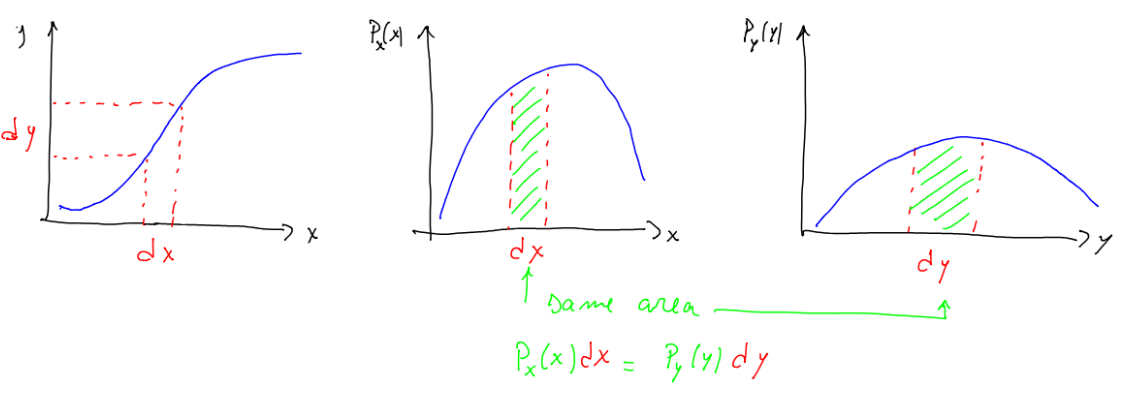
\includegraphics[width=0.8\textwidth]{image001.png}
    \caption{If $y=f(x)$ is invertible on its range, then it is either strictly increasing or decreasing. This means that the preimage $f^{-1}(I)$ of an interval $I = [y, y+\dd{y}]$ is again an \textit{interval} $J=[x, x+\dd{x}]$. Clearly, the probability of $y$ being in $I$ (which is the area in the central graph) must be the same of the probability of $x$ being in $J$ (the area in the graph to the right). By equating these two areas, we can derive formula (\ref{eqn:change-of-var-special}).\label{fig:graphical-change}.}
\end{figure}

\subsection{Generating probability distributions}
Changes of random variables can be used to \textit{simplify} the problem of sampling from a certain pdf. For example, suppose we are able to efficiently generate random numbers that are \textbf{uniformly} distributed between $0$ and $1$, and that we denote with $Y \sim \mathcal{U}([0,1])$, with:
\begin{align} \label{eqn:unif}
    p_y(y) = \begin{cases}
        1 & y \in [0,1]\\
        0 & \text{otherwise}
    \end{cases} = \mathbb{I}_{[0,1]}
\end{align}

We would like to determine a transformation $f(x)$ such that $X$ has an exponential distribution:
\begin{align}\label{eqn:exp1}
    p_x(x) = a e^{-a x} \theta(x) \qquad a > 0
\end{align} 

Using formula (\ref{eqn:change-of-var-special}) we impose:
\begin{align*}
    \left| \dv{y}{x} \right| p_y(y) \underset{(\ref{eqn:unif})}{=} \left|\dv{y}{x} \right| = p_x(x) = a e^{-ax}
\end{align*}
Then the desired transformation $f(x) \equiv y(x)$ can be obtained by integrating and inverting:
\begin{align*}
    y(x) = e^{-ax} \Rightarrow x=-\frac{1}{a} \ln y 
\end{align*}
Since $y \in [0,1]$, we have that $x \geq 0$. Thus, if we generate $y_i$ uniformly in $[0,1]$, and then apply:
\begin{align*}
    x_i = -\frac{1}{a}  \ln y_i
\end{align*}
the resulting $x_i$ are distributed according to (\ref{eqn:exp1}).

\begin{exo}[Inverse transform method]
    If $Y \sim \mathcal{U}([0,1])$, find the transformation $f$ such that:
    \begin{enumerate}[label=\alph*.]
        \item $p_x(x) = x^{-2} \mathbb{I}_{[1,\infty)}(x)$
        \item $p_x(x) = |\beta| x^{\beta-1} \mathbb{I}_{[1, \infty)}(x)$, with $\beta < 0$
        \item $p_x(x) = \beta x^{\beta-1} \mathbb{I}_{(0,1]}(x)$, with $\beta > 0$
        \item $\displaystyle p_x(x) = \frac{1}{1+x^2} \frac{1}{\pi}$ (\textbf{Cauchy's distribution}), with $Y \sim \mathcal{U}([-\pi/2, \pi/2])$.  
    \end{enumerate}
    
\end{exo}

\end{document}
